\section{Problem 2}
\textit{A large 20m high building is approximated by a screen. Use UTD eq 3.3.21 to find the additional pathloss relative to free space in the shadow region 10 meters behind the building at 1800 and 5200 MHz. Assume X large (eq.3.3.18). The base station is assumed far away.}\\

\textit{Use Matlab to plot the result.}\\

\textit{Assume a dipole as a receiving antenna. What is the difference between 1800 and 5200 MHz, when also the antennas are taken into account.}\\


Using the equation given in the literature

\begin{flalign}
E_{D_2}=- E_0 \cdot \frac{ \exp(-jk(s+s_1)) }{ \sqrt{k (s+s_1)} }  \cdot  \sqrt{\frac{1}{s s_1}} \cdot  \frac{\exp\left(\frac{-j \pi}{4} \right)}{ 2 n\sqrt{2\pi} } \cdot  \cot\left(\frac{\epsilon}{2 n}\right)
\end{flalign}

the diffracted electrical field can be calculated for different mobile terminal heights. This is done using the given Matlab template for both frequencies and can be seen in \figref{fig:MM10efield}.

\begin{figure} [!h]
\centering
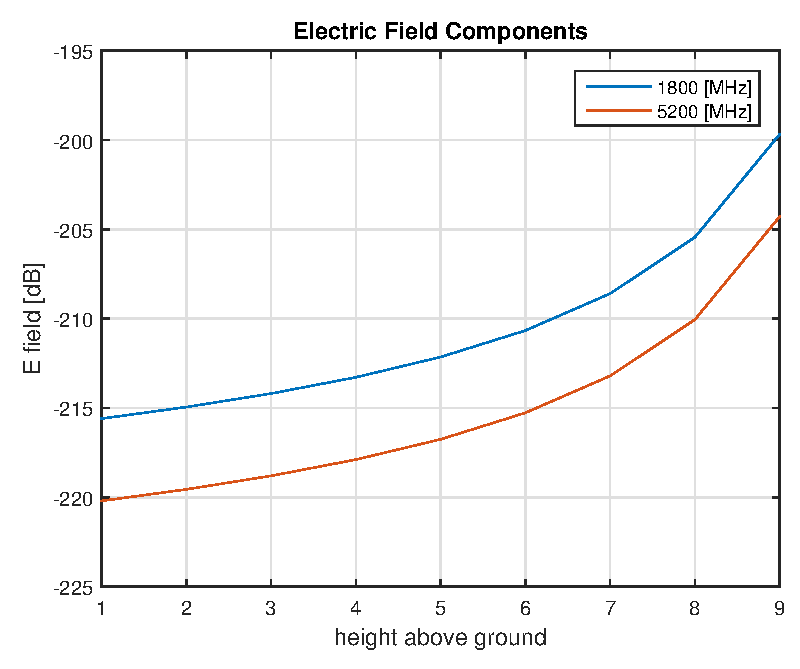
\includegraphics[width=14cm]{figures/mm10_e_field.eps}
\caption{E-Field.}\label{fig:MM10efield}
\end{figure} 

The total electrical field is only consisting of the diffracted field, since the field received by geometrical optics is zero in the shadow region. It can be seen, that the field, when the receiver is positioned further in the shadow region (lower height) is decreasing. Also, a higher frequency yields an overall lower field for all heights due to the $1/\sqrt{k} \propto 1/\sqrt{f} $ dependency. 

To calculate the power received by the antenna, the effective area of the antenna has to be considered. Depending on the gain, the effective area is

\begin{flalign}
A_e = g \frac{\lambda^2}{4\pi}
\end{flalign}

The power can be calculated by using the area and the poynting vector $S$ which can be calculated by

\begin{flalign}
&& S &= E \times H^* &\\
&& &= \eta \lvert E \rvert^2
\end{flalign}

Using a gain of \SI{1.5}{\decibeli} we can calculate the power as shown in \figref{fig:MM10power}. Again, we can see the behaviour as described above for the electric field. The two frequencies are even further apart, since we now have a $1/f^3$ dependency, which relates to a \SI{13.8}{\decibel} ($\approx 30 \Delta\left(\log_{10}(f)\right)$ with the two frequencies 1800 and 5200 MHz) difference in the power for the two calculated frequencies.

\begin{figure} [!h]
\centering
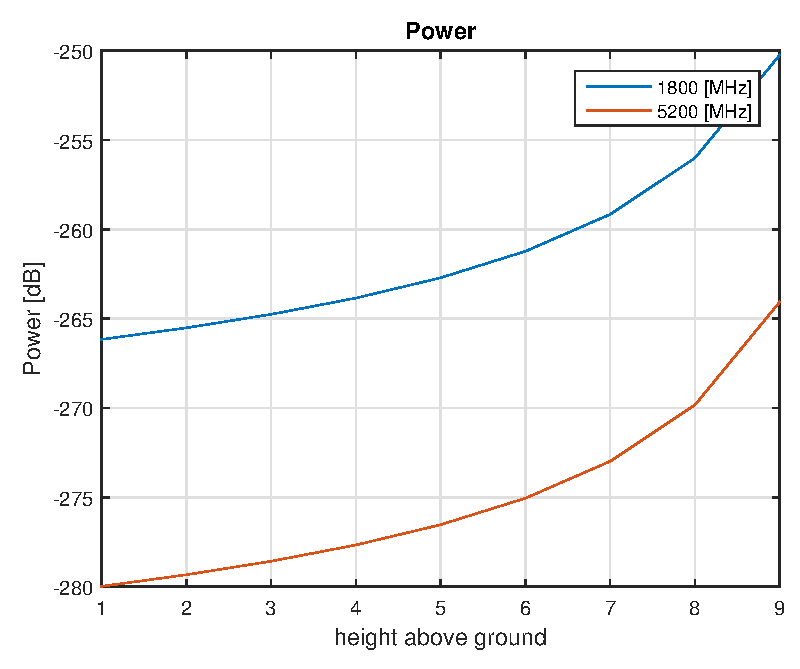
\includegraphics[width=14cm]{figures/mm10_power.eps}
\caption{Power.}\label{fig:MM10power}
\end{figure}

Depending on the actual used antenna, the gain and thus the effective area would be different and also the power would of course then be influenced by it.


